\documentclass{article}

% Language
\usepackage[english]{babel}

% Page layout
\usepackage[a4paper, top=2.5cm, bottom=2.5cm, left=3cm, right=3cm, marginparwidth=1.75cm]{geometry}

% Packages
\usepackage{amsmath}
\usepackage{float}
\usepackage{amssymb}
\usepackage{graphicx}
\usepackage{booktabs}
\usepackage{caption}
\usepackage{subcaption}
\usepackage{hyperref}
\usepackage{xcolor}
\usepackage{listings}
\usepackage{parskip}
\usepackage{microtype}
\usepackage[]{hyperref}

% Code listing style
\lstdefinelanguage{Julia}{
  keywords={using, import, function, end, if, else, elseif, for, while, return,
            const, begin, module, export, struct, mutable, abstract, type,
            @kernel, @index, @views, @., true, false},
  sensitive=true,
  comment=[l]{\#},
  morestring=[b]",
}
\lstset{
  language=Fortran,
  basicstyle=\ttfamily\small,
  keywordstyle=\color{blue}\bfseries,
  commentstyle=\color{gray}\itshape,
  stringstyle=\color{orange!80!black},
  backgroundcolor=\color{gray!8},
  frame=single,
  framerule=0.4pt,
  rulecolor=\color{gray!40},
  breaklines=true,
  showstringspaces=false,
  tabsize=4,
  captionpos=b,
  numbers=left,
  numberstyle=\tiny\color{gray},
  numbersep=6pt,
}

% Simple TODO marker -- search for "TODO" to find every open item.
\newcommand{\todo}[1]{\textcolor{red}{\textbf{[TODO: #1]}}}

\begin{document}

% Titlepage
\begin{titlepage}

% Logo top-left
\begin{flushleft}

\includegraphics[trim={0 0 0 4cm}, clip, width=4cm]{figures/EHTZ square.png}
\end{flushleft}

\centering

\textbf{Project report}\\
High Performance Computing for Weather and Climate, ETH Zürich\\

\vspace{2cm}
{\LARGE \textbf{Communication strategies for halo-updates}}\\[3em]

\begin{figure}[h!]
    \centering
    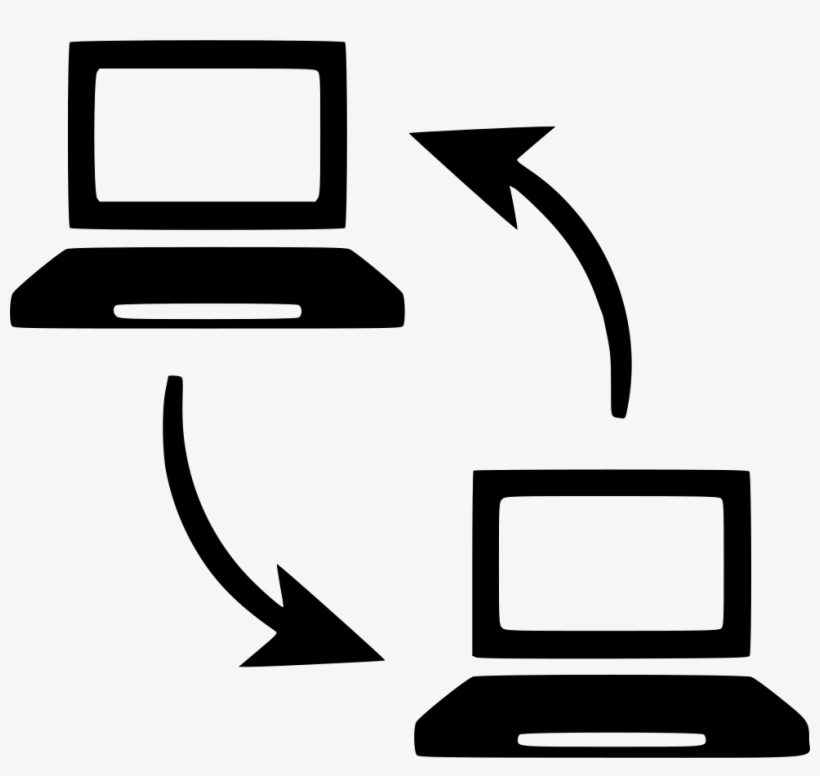
\includegraphics[width=0.5\linewidth]{figures/communication.jpeg}
\end{figure}

\vspace*{2cm}
\textbf{Authors}\\
Nico Jungck, 21-923-982\\
Ida Vetsch, 20-934-031\\
Till Wenke, 25-931-163\\


\vspace{1cm}
\textbf{Advisor}\\
Max Harvey\\

\vspace{2cm}
\today

\end{titlepage}


\newpage
\begin{abstract}
Halo exchange can limit the parallel performance of stencil computations
in weather and climate models. This report compares blocking and
non-blocking communication, overlap of communication with computation,
and explicit corner exchange for a fourth-order diffusion stencil.
The implementations are validated against a serial reference and
assessed through strong- and weak-scaling experiments on the Santis
supercomputer with up to 96 MPI ranks. Non-blocking communication
performs best among the communication-ordering strategies, while
blocking schemes with long sequential dependencies scale poorly.
Overlapping communication with computation reduces waiting time but
does not consistently improve total runtime in the tested configurations.
Explicit corner exchange reduces halo-exchange time by up to
approximately 15\% at high rank counts. Overall, the results highlight
the benefit of reducing sequential waiting, while showing that additional
overhead can offset the gains from communication optimizations.
\end{abstract}

\newpage
\tableofcontents
\newpage

% ─────────────────────────────────────────────────────────────────
\section{Introduction}
\label{sec:introduction}

Stencil-based weather and climate code is highly parallelizable, offering potential for scaling on supercomputers. This introduces the new problem of communication between processing units that don't have shared memory access. Halo exchange is the dominant communication pattern in stencil computations on a grid. At every timestep, each rank must send the data on the boundary of its subgrid to, and receive respective boundaries from, its neighbor ranks on the grid before computation can proceed. How this communication is implemented is a technical choice that can affect performance.

The task evolves a field of size $n_x\times n_y\times n_z$ for
\texttt{num\_iter} diffusion iterations. For $P$ MPI ranks, the code
chooses the closest factor pair $P_xP_y=P$ to form a two-dimensional
process grid, partitions $n_x$ across $P_x$ and $n_y$ across $P_y$, and
keeps the full $n_z$ extent on every rank.


This report investigates three largely independent design questions
for the halo exchange step of a 4th-order diffusion stencil
(\texttt{stencil2d}):

\begin{enumerate}
    \item \textbf{Blocking and non-blocking communication.} Blocking
    \texttt{Send}/\texttt{Recv} calls between neighboring ranks can deadlock. We compare three ways of avoiding this, library-managed ordering (\texttt{Sendrecv}), a checkerboard two-coloring of the process grid (\texttt{sendrecv\_evenodd}), and a cycle-breaking
    scheme that does not require a two-coloring (\texttt{brokencycles}), against a non-blocking reference (\texttt{Irecv/Isend}). We are especially interested in whether the explicit communication ordering in \texttt{sendrecv\_evenodd} and \texttt{brokencycles} behaves differently from the library-managed approaches.
    \item \textbf{Overlap of computation and communication.} In principle, non-blocking communication allows the interior of the domain (which does not depend on halo data) to be computed while halo messages are in flight. We test whether this pays off in practice.
    \item \textbf{Explicit corner exchange.} The stencil used here
    applies the Laplacian operator twice per timestep, which makes
    diagonal (corner) neighbor data relevant two grid points away. A communication strategy that is simple in the way that each grid cell only has to communicate to its direct neighbors is the sequenced top/bottom-then-left/right exchange. However this comes at the cost of additional synchronization points. We test whether explicitly exchanging corner data with diagonal neighbors improves performance, where communication does not need to happen sequentially.
\end{enumerate}


\section{Methods}
\label{sec:methods}

\subsection{Blocking and Non-Blocking Communication}
\label{sec:strategies}

All strategies in this section are implemented in
\texttt{stencil2d-comm\_strats\_timer.F90}, selected at runtime via the
\texttt{--comm\_strategy} flag. \texttt{stencil2d-comm\_strats\_timer.F90} is structured such that the sole variable between strategies is the communication mechanism; that is, all methods share identical packing, buffer management, and top/bottom, left/right sequencing.

\begin{itemize}
    \item \textbf{\texttt{Irecv/Isend}} (reference): both the send and
    the receive are posted non-blocking. This is deadlock-free by construction, since no call blocks waiting for a peer. Note that \texttt{MPI\_Waitall} is called inside the halo-update routine, before it returns. Hence, there is no overlapping communication and computation.
    \item \textbf{\texttt{sendrecv}}: a single blocking
    \texttt{MPI\_Sendrecv} call per direction pair. This is deadlock-free by construction, since the MPI library internally sequences the send
    and receive.
    \item \textbf{\texttt{Irecv/Send}}, \textbf{\texttt{Isend/Recv}}:
    receives are posted non-blocking while sends are blocking (or vice
    versa). Included as intermediate points between the fully blocking
    and fully non-blocking extremes.
    \item \textbf{\texttt{sendrecv\_evenodd}}: plain blocking
    \texttt{Send}/\texttt{Recv}, deadlock-avoided by a checkerboard two-coloring of the process grid: The ranks are placed on a process grid and each rank's color is $(\text{row} + \text{col}) \bmod 2$; color-0 ranks send to neighbors first and then receive, color-1 ranks do the reverse. For this method to work, every pair of adjacent ranks on the process grid must have opposite colors. This is guaranteed for all interior ranks by definition. However, due to the circular dependence structure, a periodic boundary condition requires that the process grid has an even number of ranks along both axes. This is a necessary and sufficient condition since from graph theory we know that a cycle has a valid two-coloring if and only if it is even.
    \item \textbf{\texttt{brokencycles}}: plain blocking
    \texttt{Send}/\texttt{Recv}, deadlock-avoided by breaking cycles of communication dependencies. The top/bottom and left/right exchanges are each split into two sequential cycles (e.g.\ ``send my top edge to my top neighbor, receive from my bottom neighbor'' as one complete cycle). Within each cycle, every rank sends first except the rank at the low end of that axis (\texttt{position(2) == 1} for top/bottom,
    \texttt{position(1) == 1} for left/right), which receives first,
    breaking the cycle and seeding a reverse cycle of receives back through the chain. Unlike \texttt{sendrecv\_evenodd}, this scheme does not require an even number of ranks along either axis, at the cost of a longer dependency chain: a message between two ranks $M$ steps apart along an axis may need $O(M)$ prior sends/receives elsewhere on that axis to resolve, whereas \texttt{sendrecv\_evenodd} resolves every neighbor pair independently in $O(1)$ steps. Hence, we expect that \texttt{brokencycles} should scale worse than \texttt{sendrecv\_evenodd} as the number of ranks grows.
\end{itemize}
We compare the performance of these strategies in Section~\ref{sec:results-blocking}, where we omit the hybrid \textbf{\texttt{Irecv/Send}}, \textbf{\texttt{Isend/Recv}} versions because of difficulty of interpretation.

\subsection{Overlapping Computation and Communication}
\label{sec:comm-comp}

\texttt{stencil2d-comm\_comp.F90} restructures the timestep loop
itself to compute the Laplacian on
the interior of the domain, the region that does not depend on halo
data, while the non-blocking halo exchange (\texttt{Irecv}/
\texttt{Isend}) is in flight, and only computes the boundary region
after the exchange completes. This strategy overlaps communication with computation.

The implementation stores the current field in \texttt{in\_field} and
uses two auxiliary arrays, \texttt{tmp1\_field} and
\texttt{tmp2\_field}. The first Laplacian is split into an interior
region and boundary regions. At the beginning of each timestep, non-blocking receives are posted for
the four neighboring faces. The corresponding send buffers are packed
and the non-blocking sends are started. The interior part of the first
Laplacian is then computed while the halo messages are in flight. Once
the required halo data has arrived, it is unpacked and the remaining
boundary regions of the first Laplacian are evaluated. The second
Laplacian is applied only after the complete intermediate field is
available.

The timestep therefore has the following logical structure:

\begin{enumerate}
    \item post the non-blocking halo exchange;
    \item compute the interior of the first Laplacian;
    \item wait for and unpack the halo data;
    \item compute the boundary of the first Laplacian;
    \item apply the second Laplacian;
    \item update the output field and copy it back for the next iteration.
\end{enumerate}


The theoretical speedup limit compared to the sequential implementation is

\begin{equation}
    S_{max} = \frac{t_{\text{comm}} + t_{\text{compute}}}{\max(t_{\text{comm}}, t_{\text{compute}})} 
    \label{eq:max-speedup}
\end{equation}

The relevant quantity in practice is the local grid size per rank. Growing the local grid makes computation scale faster than halo communication, so communication shrinks as a share of total runtime; hiding it then buys progressively less, and the speedup approaches one. Shrinking the local grid at fixed global size, e.g. by adding ranks, has the opposite effect: communication becomes proportionally more significant and the potential benefit of overlap grows, up to the point where communication dominates and there is too little computation left to hide it. Adding nodes mainly changes communication latency and network overhead and does not by itself guarantee a speedup. This bound is optimistic for two reasons. First, only the interior computation can overlap with communication; the boundary computation is on the critical path and must wait for the halo data regardless. Second, packing, unpacking, request management, synchronization, and the field update all add overhead that has no counterpart in the sequential version. Reducing communication wait time is therefore necessary but not sufficient for reducing total runtime.


\subsection{Explicit Corner Exchange}
\label{sec:corners}

The diffusion stencil applies the 5-point Laplacian operator twice per
timestep. Because the second application reads neighboring
values of the \emph{already-differenced} first-pass field, a point near
a subdomain's edge can depend on data that is diagonally adjacent on
the original grid -- which is why the halo width is $2$ rather than
$1$. The baseline strategies (Section~\ref{sec:strategies}) handle this
implicitly: the top/bottom exchange is completed and unpacked
\emph{before} the left/right exchange is packed, so left/right messages
already carry the correct diagonal corner data along for free, without
any additional messages. This adds synchronization: the left/right
exchange cannot begin until the top/bottom exchange has completed. We
assume that this sequential dependency can become a bottleneck because
each rank must wait for its top/bottom neighbors before it can start
sending to its left/right neighbors. We propose a different explicit corner exchange strategy where ranks that are responsible for diagonally adjacent grid cells communicate with each other to exchange the corners of the halo.

\paragraph{A simple model of the halo update.}
To understand the possible delay, we split each halo update into four
steps: packing data into send buffers, posting the MPI calls, transferring
the data, and unpacking the received data. The model makes four simplifying
assumptions:

\begin{enumerate}
    \item Packing, posting, and unpacking require the same total work in
    every strategy.
    \item The same total amount of data is transferred; corner values
    either travel inside the left/right messages or in separate diagonal
    messages.
    \item A transfer can start only after both ranks have posted the
    matching send and receive.
    \item The slowest rank determines the halo-update time because all
    ranks need complete halos before continuing.
\end{enumerate}

Under these assumptions, explicit corner exchange can only save time by
removing the delay between the top/bottom and left/right phases. It posts
all edge and corner messages together, so a fast rank does not have to
wait for a neighbor to reach a later communication phase.

We benchmark three explicit-corner strategies. All exchange data with
the four edge and four diagonal neighbors in one communication phase,
removing the dependency between the top/bottom and left/right exchanges:

\begin{itemize}
    \item \textbf{\texttt{corners}}
    (\texttt{stencil2d-mpi-corners.F90}): pack and post all eight
    exchanges, complete them with one \texttt{MPI\_Waitall}, then unpack.
    \item \textbf{\texttt{corners-pipelined}}
    (\texttt{stencil2d-mpi-corners-pipelined.F90}): send-side
    pipelining. Pre-post the receives, then post each group of sends as
    soon as it is packed, overlapping early transfers with later packing.
    \item \textbf{\texttt{corners-waitany}}
    (\texttt{stencil2d-mpi-corners-waitany.F90}): receive-side
    pipelining. Use \texttt{MPI\_Waitany} to unpack each halo as it
    arrives, overlapping early unpacking with later transfers.
\end{itemize}

Figure~\ref{fig:corner-model} illustrates the expected timing effect of
removing the phase dependency and of the two forms of pipelining.

\begin{figure}[H]
    \centering
    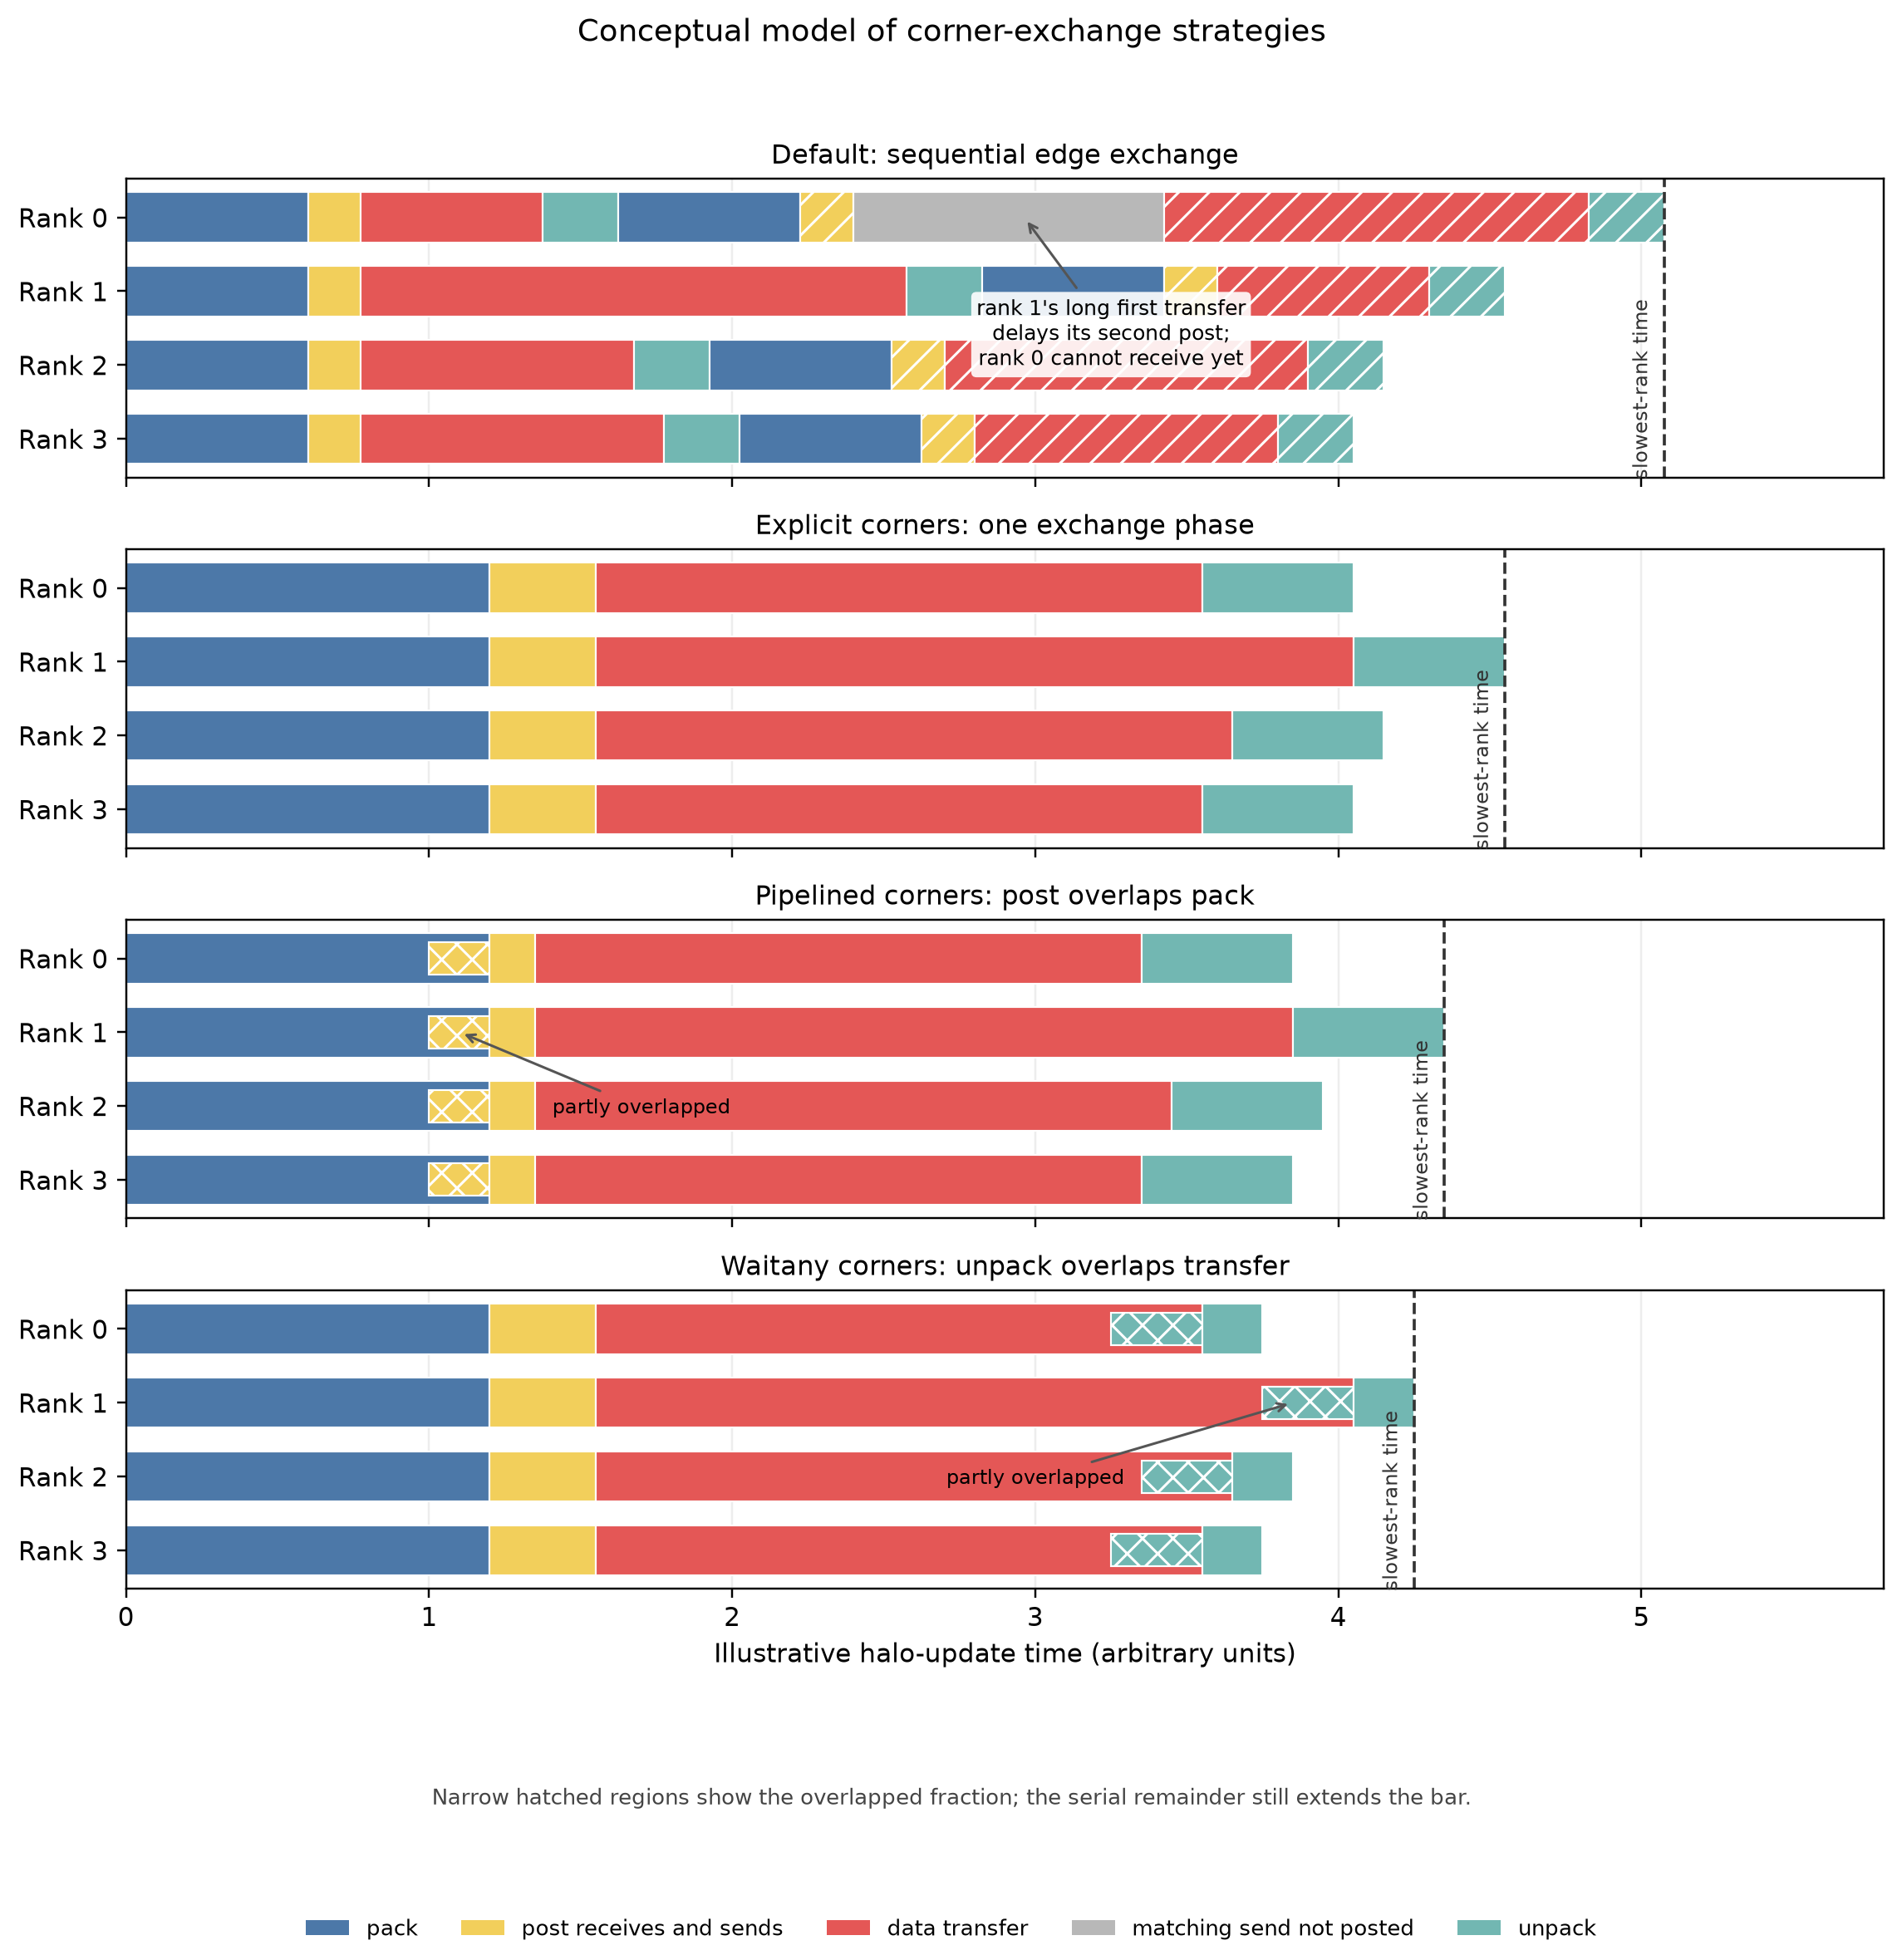
\includegraphics[width=\linewidth]{figures/corner_exchange_timing_model.png}
    \caption{Illustrative four-rank timing model for the baseline and three
    explicit-corner strategies; hatched regions denote overlapped work. For "Pipelined corners" we would also expect the transfer to overlap packing.}
    \label{fig:corner-model}
\end{figure}

We compare these variants with the non-blocking \texttt{mpi (stencil2d-mpi.F90)} baseline.

\subsection{Validation}
\label{sec:validation}

All communication strategies were validated for correctness before any
performance measurement, by comparing the full output field against a
serial reference implementation (\texttt{stencil2d-orig.F90}) using
\texttt{compare\_fields\_f90.py} at $n_x = n_y = 128$, $n_z = 4$,
$1024$ iterations, $16$ ranks on 4 Santis nodes (4 ranks per node, one
GH200 per rank).

\texttt{validation/validate\_all\_strategies.sh} runs all eight strategies this way:
the four runtime-selected ones
(\texttt{sendrecv}, \texttt{sendrecv\_evenodd}, \texttt{brokencycles}, \texttt{irecvisend}), the three
corner variants (\texttt{corners}, \texttt{pipelined},
\texttt{waitany}), and the overlap variant (\texttt{comm\_comp}). All pass at
\texttt{rtol} $=$ \texttt{atol} $= 10^{-4}$ and all eight implementations produce bit-identical output fields.


\begin{figure}[H]
    \centering
    \begin{subfigure}{0.4\textwidth}
        \centering
        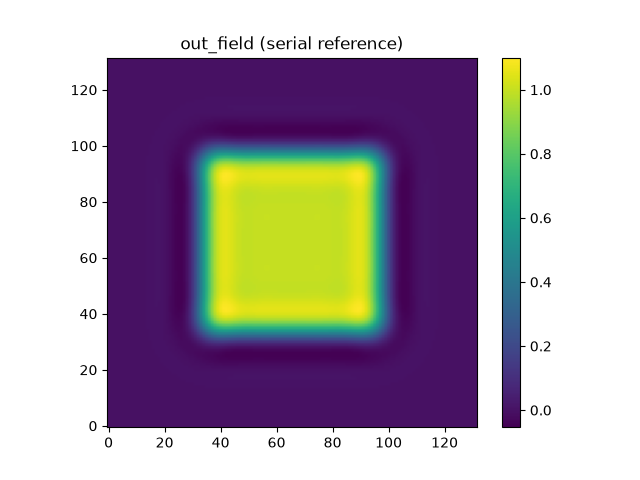
\includegraphics[width=\linewidth]{figures/out_field_ref_f90.png}
        \caption{Serial reference}
    \end{subfigure}
    \hspace{0.04\textwidth}
    \begin{subfigure}{0.4\textwidth}
        \centering
        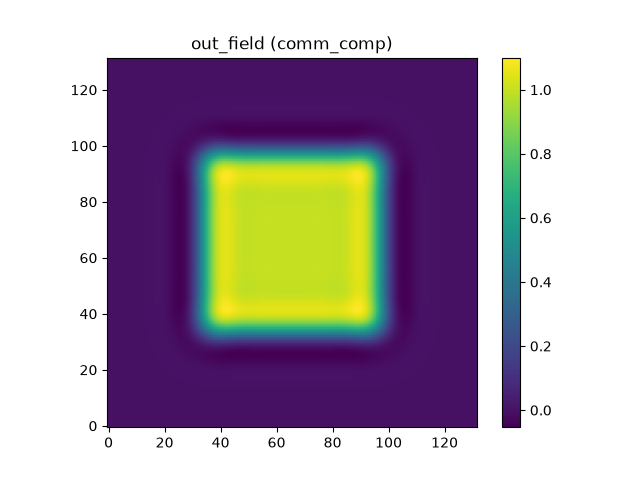
\includegraphics[width=\linewidth]{figures/out_field_comm_comp.png}
        \caption{\texttt{comm\_comp} output}
    \end{subfigure}
    \caption{Exemplary output-field heatmaps used for validation.}
    \label{fig:validation-fields}
\end{figure}

\subsection{Experimental Setup}
\label{sec:setup}

We study both weak and strong scaling. In both regimes we vary
only the number of MPI ranks and the global domain dimensions required
by the scaling definition; the numerical method, $n_z=64$, the iteration
count, and the placement policy remain fixed between strategies.

\textbf{Weak scaling.} The domain grows proportionally with the rank
count, holding the local subdomain size constant at $128\times128\times
64$ grid points per rank. For each rank count, the launcher chooses the
most nearly square two-dimensional process grid and sets the global
$n_x$ and $n_y$ accordingly. Weak-scaling efficiency is the runtime at
the smallest common rank count divided by the runtime at each larger
rank count.

\textbf{Strong scaling.} The domain is fixed at $1024 \times 1024$
with $n_z=64$, while the number of ranks increases. Strong-scaling
speedup is measured relative to the smallest common rank count and is
compared with ideal linear speedup.

The benchmark sweep runs were performed using
\texttt{experiment\_scaling\_all\_strategies.sh}.
Each Santis node contains four GH200 modules. We place exactly one MPI
rank on each GH200, request $\lceil N/4\rceil$ nodes for $N$ ranks, and use at most four ranks per node. Each rank is assigned one GPU, one CPU core. Runs with up to four ranks therefore communicate only within one node. Beginning
at five ranks, the job spans multiple nodes and at least some halo
messages cross the inter-node network. Because inter-node transfers are
substantially slower than communication between GH200 modules within one
node, the measured halo-exchange time is then expected to be dominated
by inter-node communication. We consequently expect a performance
discontinuity or slowdown at this placement boundary, in addition to the
scaling behavior caused by changing the workload per rank.

Each case uses 1024 iterations and is repeated three times. We measure
the mean diffusion-loop elapsed time across ranks as the application-level performance
metric. To explain differences between strategies, we additionally
record the average and maximum communication and computation times
across ranks. Here communication time is the time spent in the
\texttt{update\_halo} routine, which is the routine rewritten for the
different communication strategies. Where finer analysis is needed, particularly for the corner variants and overlapping computation and communication, the timing is further
separated into packing and unpacking, posting sends and receives, and
waiting for MPI requests to complete. These component timings distinguish
network or synchronization costs from local buffer-management overhead.

\section{Results}
\label{sec:results}

The commands used to obtain our results and plots can be found in our project's code repository.

\subsection{Blocking and Non-Blocking Communication}
\label{sec:results-blocking}

This section compares \texttt{sendrecv}, \texttt{sendrecv\_evenodd}, and \texttt{brokencycles} against the \texttt{irecvisend} reference, isolating the effect of how a deadlock-free ordering of communication is achieved, independent of the overlap and corner-handling questions addressed in Sections~\ref{sec:results-overlap}--\ref{sec:results-corners}.


\subsubsection{Weak Scaling}
\label{sec:results-ordering-weak}

In a weak-scaling experiment, the amount of work given to each rank is held fixed, and the total problem size grows only because more ranks are added. If communication were free, total runtime should therefore stay perfectly flat as rank count increases. Figure \ref{fig:weak-comm-compute} confirms this is exactly what happens. The orange bars represent the average time spent on computation in the experiments and stay essentially constant across all rank counts and strategies. The small variations are explained by run-to-run noise. This confirms that any difference in runtime between strategies is coming from communication.

\begin{figure}[htbp]
    \centering
    
\includegraphics[width=1\textwidth]{figures/comm_vs_compute_avg.png}
    \caption{Average communication vs.\ computation time per strategy, weak scaling ($128\times128$ local domain per rank, $n_z=64$, 4 ranks per node). We omit measuring the time to copy fields in between diffusion steps.}
    \label{fig:weak-comm-compute}
\end{figure}

Figure~\ref{fig:weak-total-time} shows the total runtime (communication and computation) against the number of ranks. The three strategies \texttt{irecvisend}, \texttt{sendrecv}, and \texttt{sendrecv\_evenodd} show similar close to flat weak scaling behavior, where \texttt{sendrecv\_evenodd} has larger initial overhead compared to the library solutions. The reference \texttt{irecvisend} seems to be the fastest strategy overall, but further testing would be necessary to see if for some settings a blocking communication pattern performs better. The \texttt{brokencycles} strategy shows clearly worse scaling behavior as predicted in Section \ref{sec:methods}, since its communication scheme becomes more expensive as more ranks are involved and the dependency chain grows. 

\begin{figure}[htbp]
    \centering
    \includegraphics[width=0.5\textwidth]{figures/total_time_scaling_weak_nico.png}
    \caption{Mean time per rank vs.\ rank count, weak scaling. Three strategies stay close to flat, \texttt{brokencycles} climbs steadily.}
    \label{fig:weak-total-time}
\end{figure}


Figure~\ref{fig:weak-efficiency} turns this into a score per rank count. Parallel efficiency is the runtime at the smallest rank count divided by the runtime at each larger rank count, so a value of $1.0$ means perfect weak scaling, indicated in the plot by the dashed 'ideal' line. This shows again that \texttt{irecvisend}, \texttt{sendrecv}, and \texttt{sendrecv\_evenodd} all stay close to the ideal line across the range tested and that \texttt{brokencycles} instead drops steadily.


\begin{figure}[htbp]
    \centering
    \includegraphics[width=0.5\textwidth]{figures/weak_scaling_efficiency_nico.png}
    \caption{Weak-scaling parallel efficiency relative to the smallest rank count (4 ranks).}
    \label{fig:weak-efficiency}
\end{figure}

A plausible explanation for why \texttt{brokencycles} degrades this way is the shape of its communication pattern as indicated in Section~\ref{sec:strategies}. Rather than every neighboring pair of ranks exchanging data independently (as the other three strategies effectively do), \texttt{brokencycles} passes the data around a ring of ranks. The first rank in the ring waits until all others have completed their communication before finally receiving its data. With more ranks joining the ring, the dependency chain grows as does the wait time of the ranks, degrading the efficiency.


A similar idea also explains the ordering we see among the
three deadlock-free strategies, not just why \texttt{brokencycles}
falls behind. \texttt{sendrecv\_evenodd} avoids deadlock using fully blocking \texttt{MPI\_Send} and \texttt{MPI\_Recv} calls, issued one at a time. Each call only returns once that single message has completely finished, so the four halo messages exchanged per phase are resolved strictly in sequence, even though the underlying network is capable of handling several messages at once. \texttt{sendrecv} does better because a single \texttt{MPI\_Sendrecv} call bundles one send and one receive together, letting the library manage that pair internally rather than forcing the program to wait for one to finish before starting the other. This halves the number of sequential waiting points compared to \texttt{sendrecv\_evenodd}. \texttt{irecvisend} goes further still: its non-blocking calls return immediately after handing a message to the network, so all four messages of a phase can genuinely overlap in hardware, and the program only waits once, for however long the slowest of the four takes, rather than for the sum of all four. This is consistent with the ordering we observe throughout Section~\ref{sec:results-blocking}.

\subsubsection{Strong Scaling}
\label{sec:results-ordering-strong}

In a strong-scaling experiment, the total problem size is held fixed and the work is split across a growing number of ranks. Each rank's share of the problem shrinks as rank count grows. The goal is for runtime to drop in proportion to the number of ranks used.

In line with the results of Section~\ref{sec:results-ordering-weak}, Figure~\ref{fig:strong-total-time} shows that \texttt{brokencycles} has the worst strong scaling behavior. The other three show similar scaling behavior with \texttt{irecvisend} seeming to perform slightly better.

\begin{figure}[htbp]
    \centering
    
\includegraphics[width=0.5\textwidth]{figures/total_time_scaling_strong.png}
    \caption{Mean time per rank vs.\ rank count, strong scaling ($1024\times1024$ domain, $n_z=64$).}
    \label{fig:strong-total-time}
\end{figure}

Figure \ref{fig:strong-speedup} shows a more interesting aspect of the strong scaling experiment. All four strategies show a superlinear speedup, that is, doubling the ranks results in a more than double speedup. As the problem is divided into smaller and smaller pieces per rank, each rank's slice can eventually become small enough to fit into the processor's cache instead of the slower main memory. This gives every rank a computation speedup on top of the benefit of simply splitting the work and more than compensating for the cost of additional communication. Note, however, that this can be called a free speedup due to hardware effects and has nothing to do with the communication strategies tested.

\begin{figure}[htbp]
    \centering
    
\includegraphics[width=0.5\textwidth]{figures/strong_scaling_speedup.png}
    \caption{Strong-scaling speedup relative to the smallest rank count (4 ranks), vs.\ ideal linear speedup.}
    \label{fig:strong-speedup}
\end{figure}



\subsection{Overlapping Computation and Communication}
\label{sec:results-overlap}

\begin{figure}[htbp]
    \centering
    
\includegraphics[width=0.5\textwidth]{figures/COMM_COMP_STRONG.png}
    \caption{Strong-scaling comparison of the computation/communication
    overlap implementation and the non-blocking \texttt{irecvisend}
    reference on a fixed $1024\times1024\times64$ domain.}
    \label{fig:comm-comp-strong}
\end{figure}

For one rank on one node with a $128\times128\times64$ grid, the measured execution time
consisted of approximately 30\% communication and 70\% computation.
The resulting upper bound for speedup is therefore approximately $1.43\times$.

This bound shrinks as the workload becomes more distributed. For eight ranks on eight nodes with a $512\times1024\times64$ grid, measured communication and computation times were approximately $0.3$ s and $3.2$ s, giving an ideal upper bound of about $1.09\times$ . The ratio remains similar even with several ranks per node, since the goal there is still to exploit the combined compute power of multiple nodes rather than to shrink the per-rank workload.

Figure~\ref{fig:comm-comp-strong} shows the strong-scaling comparison
between \texttt{comm\_comp} and the non-blocking
\texttt{irecvisend} reference. The global domain is kept fixed while
the rank count increases from 1 to 64 with 4 ranks per node. The two implementations exhibit
similar scaling, but \texttt{comm\_comp} does not outperform the
reference at any tested rank count. 

The weak-scaling experiments showed the same qualitative behavior:
\texttt{comm\_comp} reduced part of the communication wait but did not
produce a consistent total-runtime improvement over
\texttt{irecvisend}.

To confirm that computation and communication were actually overlapping in \texttt{comm\_comp}, we ran communication diagnostics with eight MPI ranks on eight nodes (one rank per node, $512\times1024\times64$  global domain, 1024 iterations). The original schedule spent approximately $0.16$\,s in the measured \texttt{middle} wait; starting the left/right exchange before the interior computation reduced this wait to between approximately $0.02$ and $0.12$\,s.


\subsection{Explicit Corner Exchange}
\label{sec:results-corners}

We benchmark the three explicit-corner strategies against the
non-blocking \texttt{mpi} baseline on Santis, scaling from 8 to 96 MPI
ranks under strong and weak scaling, with identical rank placement
throughout. We start at 8 ranks because Santis runs four ranks per
node, so every configuration spans at least two nodes and exercises
inter-node communication.

Figures~\ref{fig:corners-comm-strong} and
\ref{fig:corners-comm-weak} compare the mean time spent in
\texttt{update\_halo} under strong and weak scaling, respectively.

\begin{figure}[htbp]
    \centering
    
\includegraphics[width=\linewidth]{figures/comm_relative_bars_strong.png}
    \caption{Corner-strategy halo-exchange time under strong scaling.}
    \label{fig:corners-comm-strong}
\end{figure}

\begin{figure}[htbp]
    \centering
    
\includegraphics[width=\linewidth]{figures/comm_relative_bars_weak.png}
    \caption{Corner-strategy halo-exchange time under weak scaling.}
    \label{fig:corners-comm-weak}
\end{figure}

At high rank counts, all explicit-corner strategies outperform the
non-blocking baseline. The standard \texttt{corners} strategy improves on
the baseline by removing the dependency between its two communication
phases. The optimized \texttt{pipelined} strategy is fastest at 64
ranks, while \texttt{waitany} is fastest at 96 ranks. Thus, once
communication spans many nodes, avoiding waits can outweigh the cost of
sending four additional corner messages. In general we focus on the behavior for a large number of ranks and we assume that the trends in speedup for increased numbers of ranks continue.

The detailed timers separate packing and unpacking, posting MPI calls,
and waiting for transfers (Appendix~\ref{app:detailed-corner-timings}).
Figures~\ref{fig:packing-strong} and \ref{fig:packing-weak} show that
packing time is similar for most strategies. It is higher for
\texttt{waitany} because the code identifies and unpacks each completed
message separately after \texttt{MPI\_Waitany}, rather than unpacking all
messages together after one \texttt{MPI\_Waitall}.

The absolute-time labels in the appendix plots show that packing and
unpacking together with MPI waiting account for most of the halo-update
time; posting sends and receives is a much smaller component. A large
relative difference in the send timer therefore has only a small effect
on the total time.

Figures~\ref{fig:sending-strong} and \ref{fig:sending-weak} show that the
\texttt{pipelined} send timer is roughly twice as large as for the other
explicit-corner strategies. This timer includes three separate
posting groups and two \texttt{MPI\_Testall} calls, after the top/bottom
and left/right groups. The calls let MPI advance messages that have
already been posted while the program prepares the remaining buffers.
Their overhead is counted as send time. In the standard strategy, data
transfer starts only after all buffers have been packed and all sends
posted; in \texttt{pipelined}, the top/bottom transfers can proceed while
the left/right and corner buffers are still being packed. Consequently,
fewer transfers remain unfinished when the code reaches
\texttt{MPI\_Waitall}, reducing the time spent waiting (Figures~\ref{fig:waiting-strong} and \ref{fig:waiting-weak}). At 64 ranks this
saving is larger than the extra posting overhead, giving
\texttt{pipelined} the lowest overall halo time.

In Figures~\ref{fig:waiting-strong} and \ref{fig:waiting-weak},
\texttt{waitany} spends the least time waiting at 96 ranks. It unpacks a
message as soon as that message arrives while other transfers continue.
At lower rank counts, the bookkeeping for handling messages one at a time
costs more than the overlap saves; at 96 ranks, the reduction in waiting
is large enough to make \texttt{waitany} fastest with an overall communication time reduction of about 15 percent compared to the baseline approach.

The same mechanism explains both weak and strong scaling. As rank
count grows, more halo traffic crosses between nodes and arrives less
uniformly, creating slack between the first and last messages.
\texttt{pipelined} exploits this by starting transfers as soon as they
are packed, and \texttt{waitany} by unpacking each message as it
arrives. Both benefit more as arrival times grow more uneven, which
is why their advantage grows with rank count. At low rank counts,
neighbors are mostly on the same node and messages arrive together, so
there is little slack to exploit and the overhead of extra \texttt{MPI} calls and
bookkeeping outweighs the benefit of these strategies.

% ─────────────────────────────────────────────────────────────────
\section{Discussion and Conclusion}
\label{sec:discussion}
Several new communication strategies for the halo exchange step of a 4th-order diffusion stencil were successfully implemented, but not all lead to a reduction of overall runtime. For many strategies, our communication models were too simplistic: the expected speedups either did not materialize or appeared only at large rank counts.

As shown in Section~\ref{sec:results-ordering-weak}, the ranking among
the deadlock-avoidance strategies tracks how much sequential waiting
each one builds into its message order, from \texttt{sendrecv\_evenodd} (one wait per message) to \texttt{sendrecv} (one wait per pair) to the non-blocking \texttt{irecvisend}, which was fastest overall. The same principle explains why \texttt{brokencycles} scales worst: its ring-based dependency chain adds no extra data or messages, only extra
sequential waiting that grows with rank count.

Two further approaches target the synchronization overhead through different mechanisms: \texttt{comm\_comp} overlaps it with computation, while \texttt{corners} removes it outright. Neither reduces the total volume of data exchanged between ranks. \texttt{corners} sends four additional messages per exchange. \texttt{comm\_comp} instead adds communication bookkeeping and splits the Laplacian computation into an interior region (computable while communication is in flight) and a boundary region (which must wait for the halo data), along with the associated request management and synchronization. Additional timers confirmed that this revised schedule successfully overlaps communication with computation, but the reduction was too small to offset the added overhead: communication wait dropped without any corresponding gain in total application runtime. Further experiments would be needed to understand the exact sources of this overhead.

\texttt{corners}, by contrast, removes a synchronization point entirely. In the baseline strategies, the left/right exchange cannot start until the top/bottom exchange has completed on \emph{every} neighboring rank, so a rank that finishes early still has to wait for its slowest neighbor before posting the next phase. \texttt{corners} eliminates this dependency by posting all eight edge and corner exchanges together in a single phase. The four additional messages are a small fixed cost, whereas the removed delay grows with rank count: for strong scaling at 64 ranks \texttt{pipelined} wins (about 11\% faster communication), and at 96 ranks \texttt{waitany} wins (about 15\% faster communication).

Our experiments suggest that minimizing waiting time is more critical than reducing message count. However, overlapping communication and computation shows that interactions are complex. Isolating and quantifying the relative impact of sequential delays versus message volume will require further testing.

Overall, the best strategy depends on domain size and rank count: our experiments favor a non-blocking \texttt{irecvisend} strategy, with \texttt{waitany} or \texttt{pipelined} becoming best only at high rank counts, while \texttt{comm\_comp}  could become beneficial on systems or workloads with a larger communication fraction and sufficient independent computation to hide it. However, no such benefit was observed in the configurations tested here.



\section{Outlook}
\label{sec:outlook}

Several directions could naturally extend this work:

\begin{itemize}
    \item Further investigation of the overhead limiting the performance of the \texttt{comm\_comp} implementation and design of an adversarial setup, where one can deliberately complete the interior computation during the halo communication.
    \item Try the communication strategies for more complex stencils, for example including vertical communication needs.
    \item Further test higher rank counts to verify if the observed trends continue and isolate the effect of intra-node communication.
\end{itemize}

\newpage

\appendix
\section{Detailed Corner-Exchange Timings}
\label{app:detailed-corner-timings}

\subsection{Packing and Unpacking}
\label{app:corner-packing}

Figures~\ref{fig:packing-strong} and \ref{fig:packing-weak} show the
packing timer used in the discussion of Section~\ref{sec:results-corners}.
The timer includes outgoing-buffer packing and received-buffer unpacking;
for \texttt{waitany}, it also includes selecting and processing each
individually completed request.

\begin{figure}[htbp]
    \centering
    
\includegraphics[width=\linewidth]{figures/packing_relative_bars_strong.png}
    \caption{Packing and unpacking time by strategy under strong scaling,
    normalized to the slowest strategy at each rank count.}
    \label{fig:packing-strong}
\end{figure}

\begin{figure}[htbp]
    \centering
    
\includegraphics[width=\linewidth]{figures/packing_relative_bars_weak.png}
    \caption{Packing and unpacking time by strategy under weak scaling,
    normalized to the slowest strategy at each rank count.}
    \label{fig:packing-weak}
\end{figure}

\subsection{Send and Receive Initiation}
\label{app:corner-sending}

Figures~\ref{fig:sending-strong} and \ref{fig:sending-weak} show the
time attributed to posting non-blocking sends and receives. For the
pipelined variant this timer additionally contains the intermediate
\texttt{MPI\_Testall} progress calls.

\begin{figure}[htbp]
    \centering
    
\includegraphics[width=\linewidth]{figures/sending_relative_bars_strong.png}
    \caption{Send/receive initiation time by strategy under strong
    scaling, normalized to the slowest strategy at each rank count.}
    \label{fig:sending-strong}
\end{figure}

\begin{figure}[htbp]
    \centering
    
\includegraphics[width=\linewidth]{figures/sending_relative_bars_weak.png}
    \caption{Send/receive initiation time by strategy under weak scaling,
    normalized to the slowest strategy at each rank count.}
    \label{fig:sending-weak}
\end{figure}

\subsection{Waiting for Communication}
\label{app:corner-waiting}

Figures~\ref{fig:waiting-strong} and \ref{fig:waiting-weak} show the
time spent inside \texttt{MPI\_Waitall} or the repeated
\texttt{MPI\_Waitany} calls. This is exposed communication latency for
which the rank cannot perform useful work.

\begin{figure}[htbp]
    \centering
    
\includegraphics[width=\linewidth]{figures/waiting_relative_bars_strong.png}
    \caption{MPI waiting time by strategy under strong scaling,
    normalized to the slowest strategy at each rank count.}
    \label{fig:waiting-strong}
\end{figure}

\begin{figure}[htbp]
    \centering
    
\includegraphics[width=\linewidth]{figures/waiting_relative_bars_weak.png}
    \caption{MPI waiting time by strategy under weak scaling, normalized
    to the slowest strategy at each rank count.}
    \label{fig:waiting-weak}
\end{figure}

\newpage
% ─────────────────────────────────────────────────────────────────
\section{Statement of AI use}
We used AI tools (LLMs) to help write code and this report. Ideas and content are our own.
\end{document}